\chapter{Risultati}
\label{chap:risultati}

Di seguito verranno mostrati i dati più significativi prodotti atraverso del codice Python. Sono state utilizzate diverse librerie, tra cui:

\begin{itemize}
    \item Pandas e Numpy, per la manipolazione dei dataset
    \item Plotly, per la visualizzazione dei dati
    \item UMAP, per la riduzione della dimensionalità dei dataset 
    \item SBO, per la generazione dei dati fuori dalla distribuzione
    \item XGBoost, il modello addestrato
    \item Scikit-learn, per la valutazione del modello e per il preprocessamento dei dati
\end{itemize}

Tutto il codice utilizzato si trova su \href{https://github.com/guglielmobartelloni/thesis-utils}{Github}~\cite{github} .

\section{Preparazione dei dati}

Come detto nel capitolo \ref{chap:generazione_di_attacchi_usando_sbo}, i dati non possono essere utilizzati come sono ma hanno bisogno di un preprocessamento. In particolare, sono stati eliminati i dati non numerici attraverso il metodo di Pandas "pandas.DataFrame.replace" come segue:


\begin{python}
input_data.replace([np.inf, -np.inf], -1, inplace=True)
input_data.replace(np.nan, -1, inplace=True)
\end{python}

Si estrae poi la colonna label dal dataset, che dovrà essere utilizzata successivamente per il modello.

Si procede poi a rinominare le etichette dei vari attacchi in "attack":

\begin{python}
attacks_packets_types = ['Bot', 'DDOS attack-HOIC', 'DDOS attack-LOIC-UDP',
                          'DoS attacks-Hulk', 'DoS attacks-SlowHTTPTest', 
                          'FTP-BruteForce', 
                          'Infilteration', 'SSH-Bruteforce']
attacks_packets.replace(attacks_packets_types, 'attack', inplace=True)
\end{python}

Si estraggono poi i pacchetti normali e quelli di attacco:

\begin{python}
normal_packets = input_data[input_data['label'] == "normal"]
attack_packets = input_data[input_data['label'] != "normal"]
\end{python}


\section{Generazione dei pacchetti}

Si è generato i nuovi pacchetti attraverso la libreria Python SBO fornita da ~\cite{sbo}. Il metodo "soft\_brownian\_offset" della libreria richiede:

\begin{itemize}
    \item i dati da cui generare i nuovi pacchetti
    \item d\_min ($d^{-}$)
    \item d\_off ($d^{+}$)
    \item softness ($\sigma$)
    \item numero di pacchetti da generare
\end{itemize}

\begin{python}
data_ood = soft_brownian_offset(data_i, d_min_, d_off_,
                                    softness=softness_,
                                  n_samples=n_ood_samples)
\end{python}


\section{Rappresentazione grafica dei dati}
 
In questa sezione esploreremo i dati generati da Soft Brownian Offset graficamente utilizzando la libreria UMAP ~\cite{umap} per ridurre la dimensionalità dei dati. . 

I test sono stati eseguiti con i seguenti parametri:

\begin{python}
umap_2d = UMAP(n_components=2, init='random', random_state=0,
               n_neighbors=70, min_dist=.8)
\end{python}

che risulta avere il giusto compromesso tra velocità e accuratezza.

Tramite la rappresentazione grafica dei dati è possibile notare in maniera chiara se i pacchetti generati sono più simili a quelli di attacco oppure a quelli normali. L'obbiettivo è quello di generare dati che siano graficamente vicini ai pacchetti di attacco ma lontani da quelli normali, questo infatti si traduce, come vedremo nelle sezioni successive, in un addestramento del modello migliore. Le tecniche di generazioni più efficaci quindi, saranno quelle che riescono a generare pacchetti non troppo distanti da quelli di attacco già presenti nel dataset.

I dati inoltre sono stati generati attraverso varie impostazioni di SBO manipolando i parametri $d^{-}$, $d^{+}$ e $\sigma$.

Analizziamo quindi i due approcci citati nel capitolo \ref{chap:generazione_di_attacchi_usando_sbo} ossia la generazione dei dati partendo da solo pacchetti normali e la generazione dei dati partendo da solo pacchetti di attacco.

\subsection{Generazione a partire dai pacchetti normali}

Questo metodo di generazione dei pacchetti, in uno scenario reale, è quello che potrebbe essere utilizzato maggiormente, in quanto solitamente non si hanno a disposizione tanti dati su attacchi informatici all'interno della propria rete, ma solo dati di traffico comune. In figura ~\ref{fig:gen_ADFA_norm_1} si nota però, come questo metodo non sia molto efficace infatti, ci sono delle evidenti sovrapposizioni tra pacchetti normali e pacchetti generati mentre, in corrispondenza degli attacchi, questo non accade. In figura ~\ref{fig:gen_ADFA_norm_2} troviamo un esempio di generazione di 25 000 pacchetti OOD e anche in questo caso, non ci sono miglioramenti. Le figure successive ~\ref{fig:gen_CICIDS_norm_1} e ~\ref{fig:gen_CICIDS_norm_2} sono invece i test eseguiti su CICIDS che ottengono i medesimi risultati.

E' evidente che i pacchetti generati, siano troppo simili ai pacchetti normali e troppo dissimili da quelli di attacco. Questa valutazione qualitativa potrebbe già darci un'idea sulla qualità di addestramento del modello.

\begin{figure}[htpb]
    \centering
    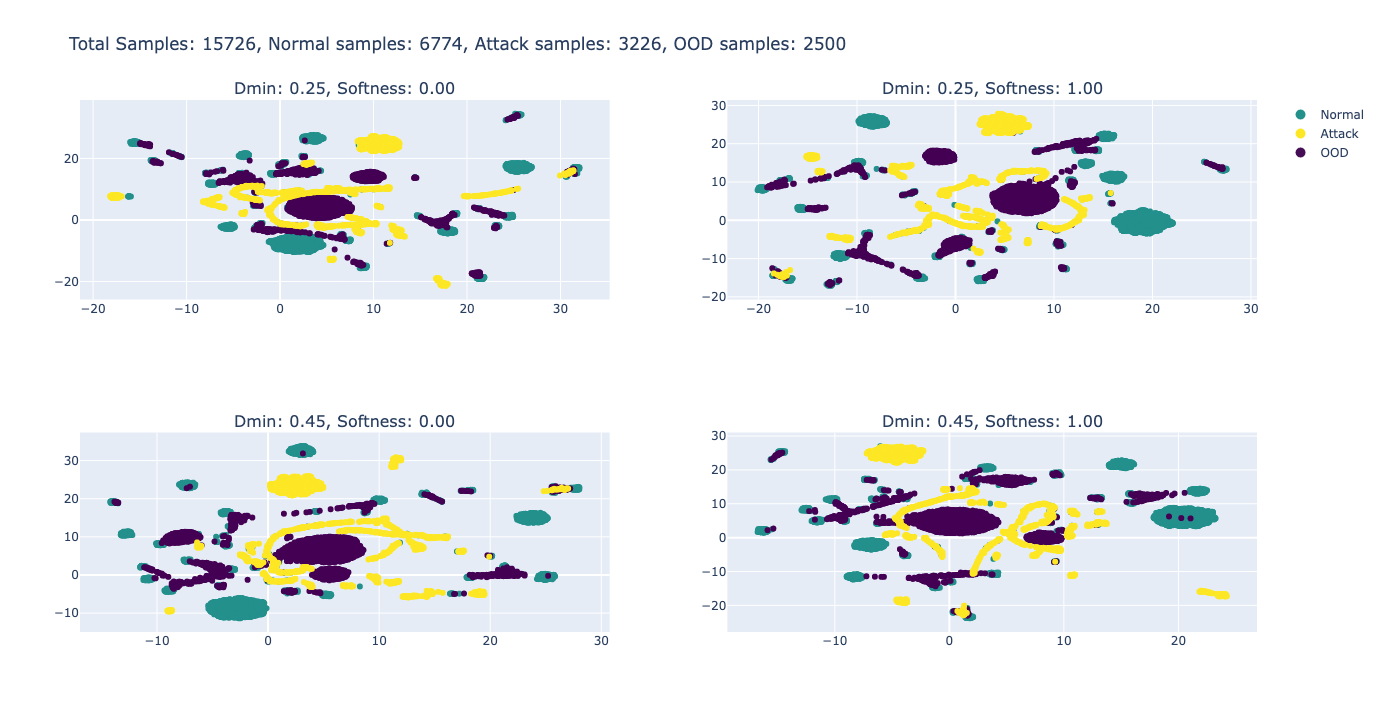
\includegraphics[width=\textwidth,height=10cm,keepaspectratio=true]{img/gen_test/adfa/ADFANET_normal_only_reduced_ood.png}
    \caption{
      (Dataset ADFANET - Generazione da normali) In giallo i pacchetti di attacco, in viola i pacchetti generati ed in verde i pacchetti normali. Questi grafici sono stati prodotti a partire da una porzione di dati ristretta per permettere una migliore visualizzazione.
    }
    \label{fig:gen_ADFA_norm_1}
\end{figure}


\begin{figure}[htpb]
    \centering
    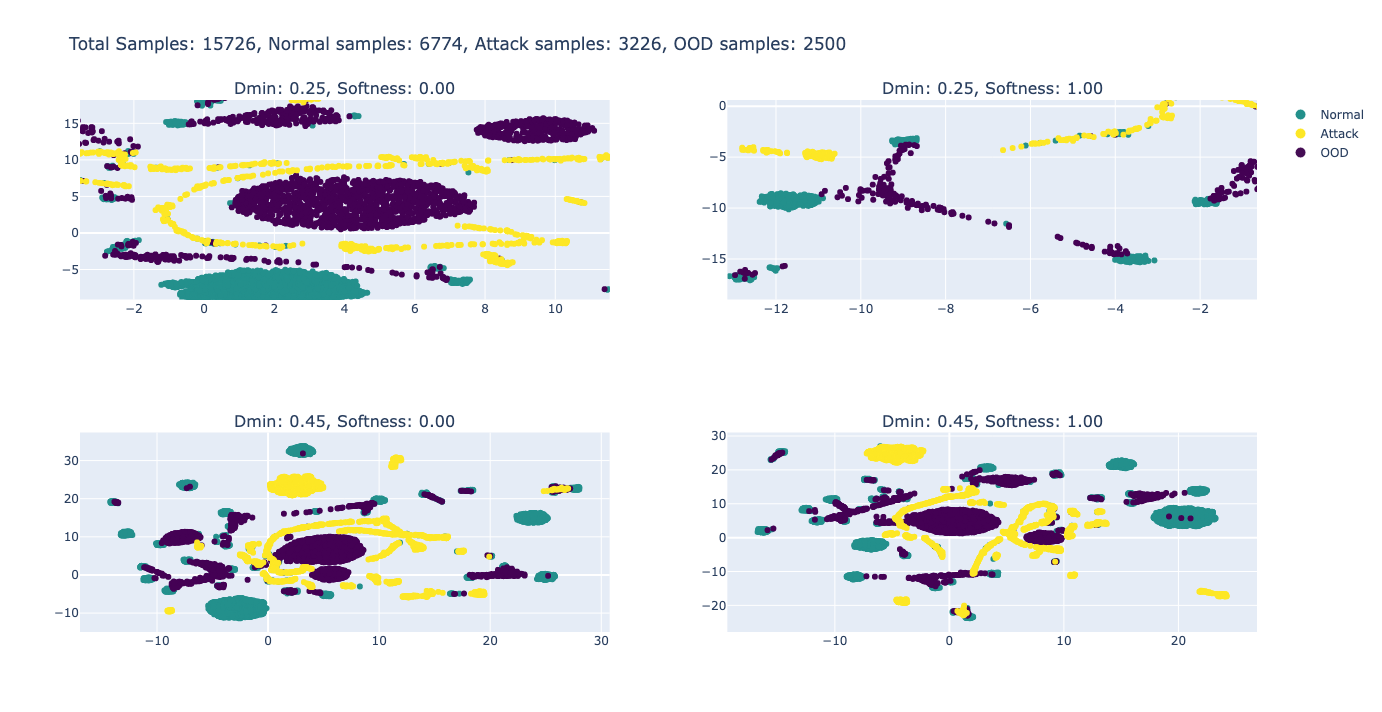
\includegraphics[width=\textwidth,height=10cm,keepaspectratio=true]{img/gen_test/adfa/ADFANET_normal_only_reduced_ood_zoomed.png}
    \caption{
      (Dataset ADFANET - Generazione da normali) Questa figura presenta i dati della figura \ref{fig:gen_ADFA_norm_1} ingranditi per permettere una migliore visualizzazione.
    }
    \label{fig:gen_ADFA_norm_1_zoomed}
\end{figure}


\begin{figure}[htpb]
    \centering
    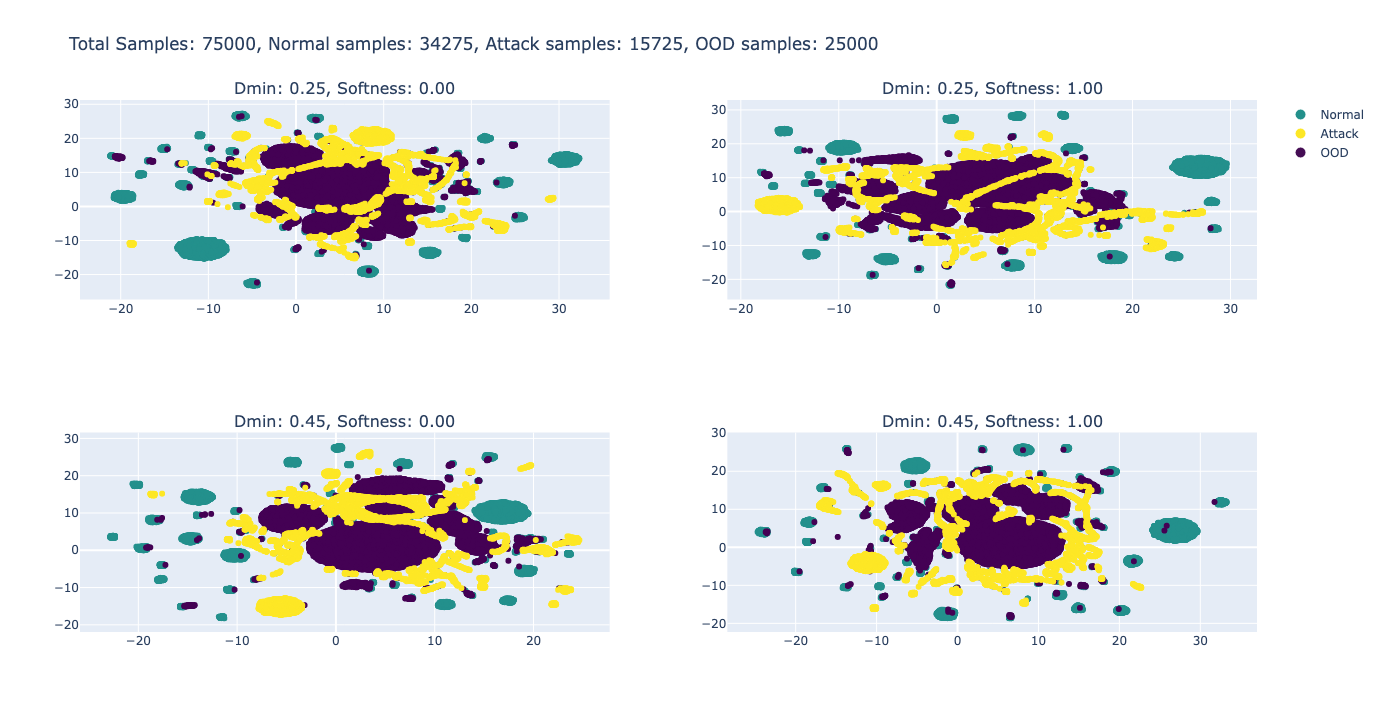
\includegraphics[width=\textwidth,height=10cm,keepaspectratio=true]{img/gen_test/adfa/ADFANET_normal_only_25k_ood.png}
    \caption{
      (Dataset ADFANET - Generazione da normali) Sono stati utilizzati 75 000 pacchetti in totale. Anche in questo caso si nota i medesimi problemi delle figure \ref{fig:gen_ADFA_norm_1} e \ref{fig:gen_ADFA_norm_1_zoomed}.
    }
    \label{fig:gen_ADFA_norm_2}
\end{figure}


\begin{figure}[htpb]
    \centering
    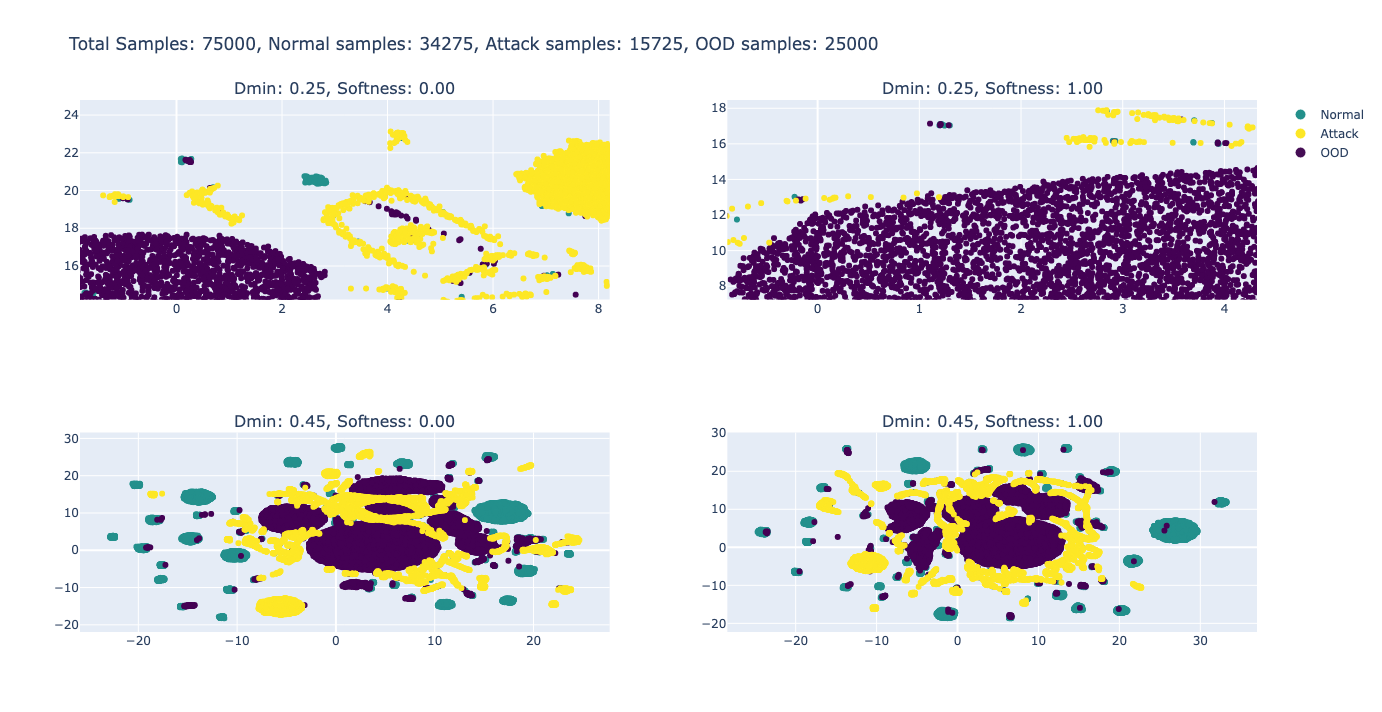
\includegraphics[width=\textwidth,height=10cm,keepaspectratio=true]{img/gen_test/adfa/ADFANET_normal_only_25k_ood_zoomed.png}
    \caption{
      (Dataset ADFANET - Generazione da normali) Versione ingrandita di \ref{fig:gen_ADFA_norm_2}.
    }
    \label{fig:gen_ADFA_norm_2_zoomed}
\end{figure}


\begin{figure}[htpb]
    \centering
    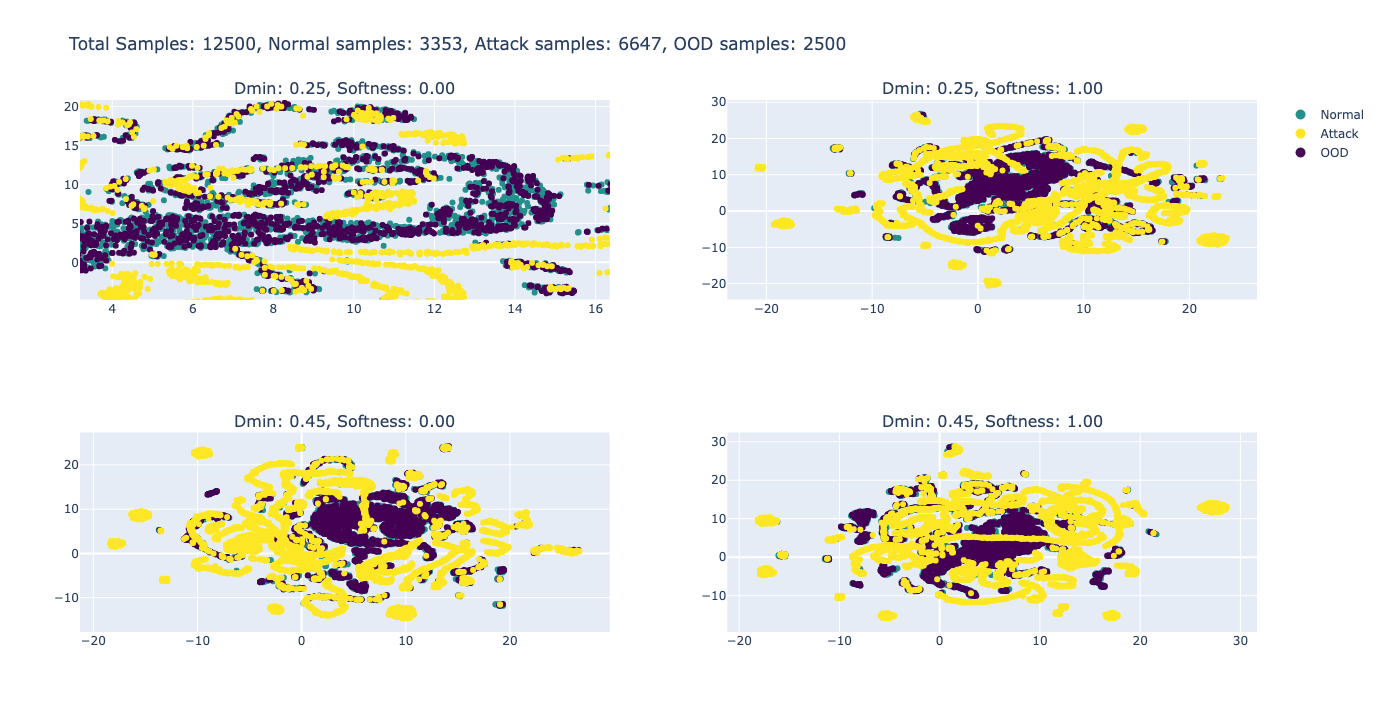
\includegraphics[width=\textwidth,height=10cm,keepaspectratio=true]{img/gen_test/cicids/CICIDS18_normal_only_25p_ood.png}
    \caption{
      (Dataset CICIDS - Generazione da normali) Si nota la maggiore complessita di questo dataset, ma si presentano gli stessi problemi di ADFANET.
    }
    \label{fig:gen_CICIDS_norm_1}
\end{figure}


\begin{figure}[htpb]
    \centering
    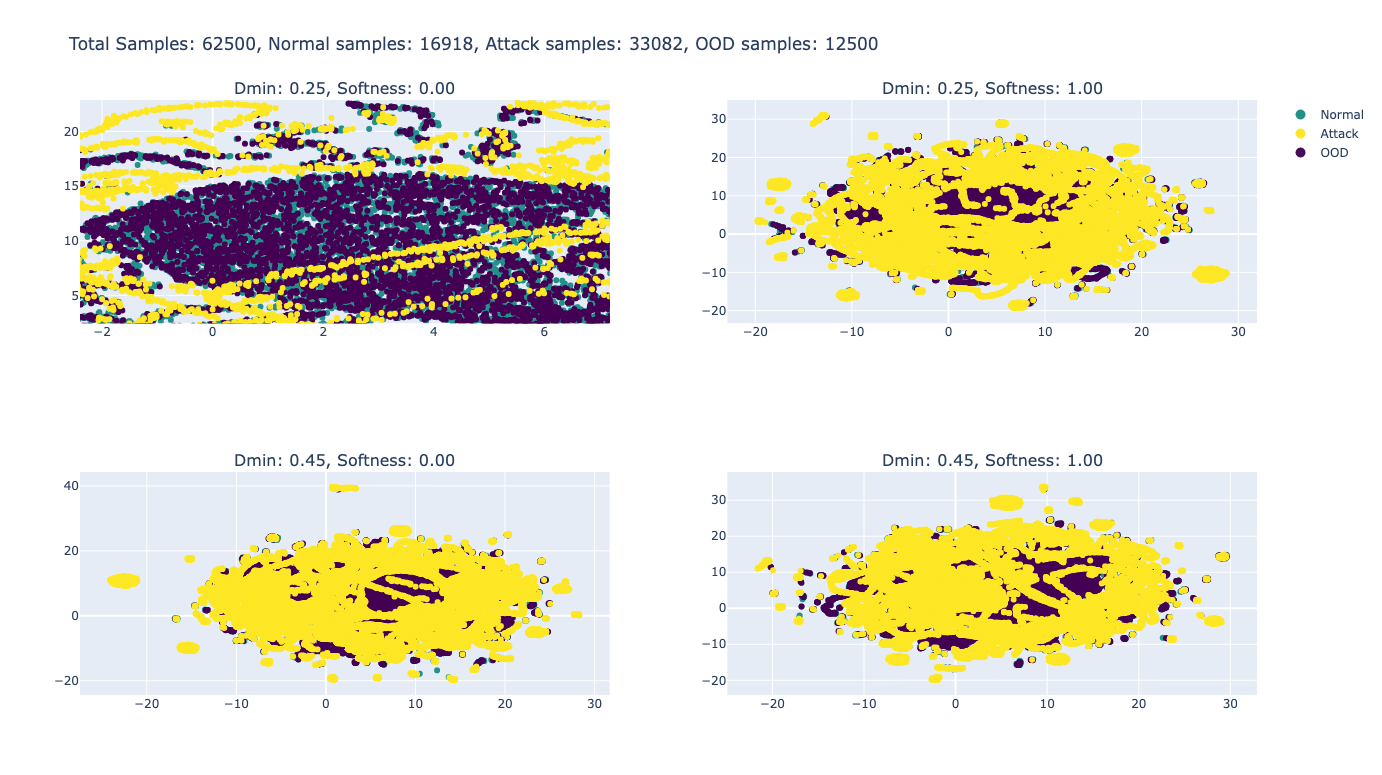
\includegraphics[width=\textwidth,height=10cm,keepaspectratio=true]{img/gen_test/cicids/CICIDS18_normal_only_12k_ood.png}
    \caption{
      (Dataset CICIDS - Generazione da normali) Questa immagine contiene grafici con più di 62 000 pacchetti. Nel grafico in alto a sinistra si nota come i pacchetti generati siano sovrapposti a quelli normali.
    }
    \label{fig:gen_CICIDS_norm_2}
\end{figure}


\subsection{Generazione a partire dai pacchetti attacco}

Questa è la modalità opposta rispetto a quella precedentemente citata, dove si generano i dati sintetici a partire dai pacchetti di attacco. Come vediamo in figura ~\ref{fig:gen_CICIDS_attack_1}, in questo caso i pacchetti OOD, sono separati dai dati normali ma vicini a quelli di attacco. Questa, osservando i grafici, sembra essere una buona soluzione di generazione, nelle sezioni successive vedremo però che anche questo metodo non è efficace per migliorare il rilevamento da parte del modello.

\begin{figure}[htpb]
    \centering
    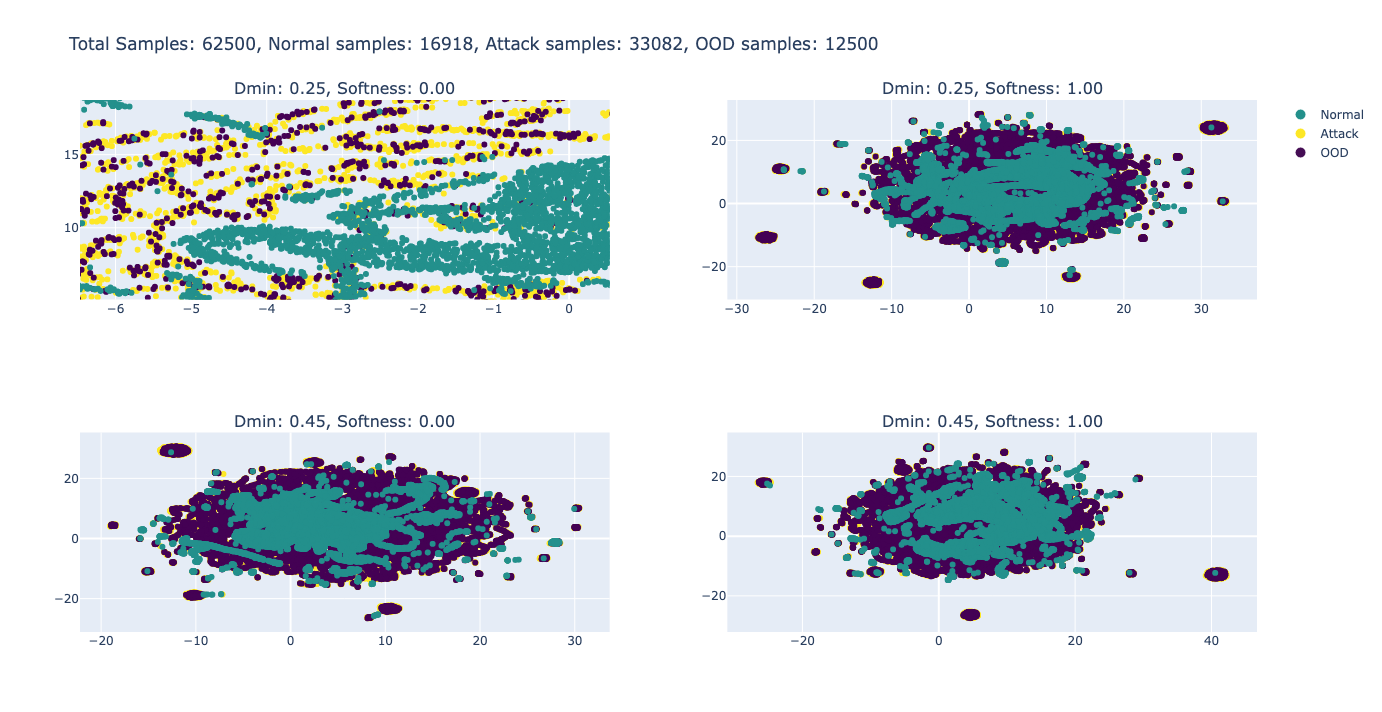
\includegraphics[width=\textwidth,height=10cm,keepaspectratio=true]{img/gen_test/cicids/CICIDS18_attack_only_12k.png}
    \caption{
      (Dataset CICIDS - Generazione da attacchi) Questa immagine contiene grafici con più di 62 000 pacchetti. Nel grafico in alto a sinistra si nota come i pacchetti generati siano sovrapposti a quelli di attacco.
    }
    \label{fig:gen_CICIDS_attack_1}
\end{figure}


\section{Addestramento del modello}

\section{Calcolo delle metriche}


